\documentclass{article}
\usepackage{amsmath}
\usepackage{amssymb}
\usepackage{graphicx}
\usepackage{lipsum}
\usepackage[margin=1in, includefoot]{geometry}
\usepackage{fancyhdr}
\usepackage{float}
\usepackage{subcaption}
\pagestyle{fancy}
\fancyhead{}
\fancyfoot{}
\fancyfoot[R]{ \thepage\ }
\renewcommand{\headrulewidth}{0pt}
\renewcommand{\footrulewidth}{0pt}
\newcommand{\Cbar}{\overline{C}}
\newcommand{\Ebar}{\overline{E}}
\newcommand{\Rg}{\ensuremath{R_\text{g}}}
\newcommand{\CRFs}{\ensuremath{\Phi_\text{s}}}
\newcommand{\PL}{\ensuremath{P_\text{l}}}
\newcommand{\TL}{\ensuremath{T_\text{l}}}
\begin{document}
	
	\begin{center}
		\huge{\bfseries Economic Analysis of using PV + Battery Setup in a Constant Load Demand}\\
		\line(1,0){300}\\
		[0.1in]
		\textsc{\LARGE BESS Techno-Commercial Project, IIT Bombay}
	\end{center}
\section{Introduction}
We are performing an economic analysis of the case when a (solar PV + battery) setup is being used to reduce the dependence of load on the grid in the most optimal way. In this case study, we assume a constant load curve (with load power P\textsubscript{L}) for time duration T\textsubscript{L} in a day. We also assume a constant grid rate R\textsubscript{g} throughout the day. 

\section{Levelised Cost Of Electricity}
Levelised cost of energy is defined as -\\
\[
\text{LCOE} = \frac{C_0 + \sum_{k=1}^{n} \frac{C_k}{(1+i)^k}}{\sum_{k=1}^{n} \frac{E_k}{(1+i)^k}}
\]

where,
\begin{align*}
	C_0 & = \text{Investment expenditure (initial capital cost)} \\
	C_k & = \text{Annual total costs (operation and maintenance) in year } k \\
	E_k & = \text{Produced quantity of electricity in the year } k \text{ in kWh} \\
	i & = \text{Real discount rate} \\
	n & = \text{Lifespan of the project (years)} \\
	t & = \text{Year of lifetime}
\end{align*}
\newline
If we assume uniform annual O\&M cost to be \(\Cbar\) and uniform annual energy savings to be \(\Ebar\), then, for discount rate 'd', we get LCOE (which is referred to as p) to be - \\
\[
\text{p} = \frac{C_0 + \Cbar \sum_{k=1}^{n} \frac{1}{(1+d)^k}}{\Ebar \sum_{k=1}^{n} \frac{1}{(1+d)^k}}
\]
\newline
\newline
Now, by using the relation
\[
\frac{1}{\Phi} = \sum_{k=1}^{n} \frac{1}{(1+d)^k}
\]
where \(\Phi\) is the Capital Recovery Factor, \\
we get LCOE as -\\
\[
\text{p} = \frac{C_0 \Phi + \Cbar}{\Ebar}
\]
If we assume \(\Cbar\) to be a fraction 'x' of C\textsubscript{0}, i.e., \(\Cbar\) = xC\textsubscript{0}, then
\begin{equation}
	\text{p} = \frac{(\Phi + x)(C_0)}{\Ebar}
\end{equation}
\vspace{10pt}
\section{Cost of Solar Energy}
For a solar PV panel setup, usually x is 0, lifespan(n) is 25 years. 
Hence, for d = 10\%, CRF(\(\Phi_\text{s}\)) comes out to be 0.11.\\
\newline
The initial cost (installation cost) of solar PV setup can be written as
$C_\text{0} = K \, P_\text{s}$ 
where
K (in Rs/kW) is the cost of installing the solar PV setup per unit capacity and
P\textsubscript{s} (in kW) is the installed capacity of solar PV setup\\
\newline 
Annual Energy Savings can be given by \(\Ebar\) = $P_\text{s} \, T_\text{s} \, d_\text{y}$ where
T\textsubscript{s} (in hr/day) is the duration of solar availability per day and
d\textsubscript{y} is the number of days of active power consumption in a year\\
\newline
Hence, by using equation (1) and by substituting the values for x to be 0,
the levelised cost for solar PV setup, which we can call as cost of solar energy R\textsubscript{s} can given as-\\
\begin{equation}
	R_\text{s} = \frac{\phi_\text{s} K P_\text{s}}{P_\text{s} T_\text{s} d_\text{y}} = \frac{\Phi_\text{s} K}{d_\text{y} T_\text{s}}
\end{equation}
We notice that the cost of solar energy is coming out to be independent of the capacity (P\textsubscript{s}) installed.\\
\newline
After substituting \(\Phi_\text{s}\) = 0.11, \(K\) = Rs. 35000/kW, \(d_\text{y}\) = 300 days, \(T_\text{s}\) = 5 hrs,\\
we get \(R\)\textsubscript{s} = Rs. 2.56/kWh

\section{Cost of Energy Storage in Battery}
During the duration of solar energy(\(T\)\textsubscript{s}), the load demand is provided by solar and the excess solar power (\(P\)\textsubscript{s} - \(P\)\textsubscript{l}) is used to charge the battery which then discharges afterwards.\\
\newline
Hence, we can define battery capacity (\(C\)\textsubscript{b}) using the following relation -
\begin{equation}
	\delta \, C_\text{b} = \eta_\text{c} \, (P_\text{s} - P_\text{l}) \, T_\text{s}
\end{equation} 
Here, \(\delta \) is the depth of discharge of the battery and \(\eta\)\textsubscript{c} is the charging efficiency of the battery.\\
\newline 
Hence, we can consider the solar + battery setup to comprise of two parts -\\
1. \textbf{Purely Solar} of capacity \(P\)\textsubscript{l}, which meets the load demand during solar duration (T\textsubscript{s})\\
2. \textbf{Solar} of capacity (\(P\)\textsubscript{s} - \(P\)\textsubscript{l}) and \textbf{Battery} of capacity $\eta_\text{c} \, (P_\text{s} - P_\text{l}) \, T_\text{s}/\delta$ \\
\newline
\newline
For the purely solar part, the cost of energy can be given by R\textsubscript{s} defined in equation (2). For, the solar + battery part, we need to define a new cost of energy R\textsubscript{b}. To calculate R\textsubscript{b}, we will use equation (1).\\
\newline
The annual energy saved/provided by this solar + battery setup is the energy finally discharged by the battery in an year, which is given by - \\
\[
    \Ebar = \eta_\text{d} \, \delta \, C_\text{b} \, d_\text{y} = \eta_\text{d} \, \eta_\text{c} \, (P_\text{s} - P_\text{l}) \, T_\text{s} \, d_\text{y} = \eta \, (P_\text{s} - P_\text{l}) T_\text{s} d_\text{y}
\]
Here,
\(\eta\)\textsubscript{d} is the discharging efficiency and
\(\eta\) is the round-trip efficiency given by \(\eta_\text{c}\)\(\eta_\text{d}\)\\
\newline
The initial cost of the setup can be given by - \\
\[
   C_\text{0} = J \, C_\text{b} + K \, (P_\text{s} - P_\text{l})
\]
Since, O\&M cost of solar is 0, we will consider only the battery for O\&M costs.\\
Hence,
\[
   \overline{C} = x \, J \, C_\text{b}
\]
Here, J (in Rs./kWh) = Initial cost of the battery per unit capacity\\
\newline
We can write R\textsubscript{b} as -\\
\[
   R_\text{b} = \frac{\Phi \, C_\text{0} +  \overline{C}}{\Ebar} = \frac{(\Phi_\text{b} + x) \, J \, C_\text{b} + \Phi_\text{s} \, K \, (P_\text{s} - P_\text{l})}{\eta \, (P_\text{s} - P_\text{l}) \, T_\text{s} \, d_\text{y}}
\]
where \(\Phi_\text{b}\) is the CRF for battery setup and \(\Phi_\text{s}\) is the CRF for solar PV setup.\\
After substituting \(C\)\textsubscript{b} from equation (3), we get final equation for \(R\)\textsubscript{b} as -\\
\begin{equation}
  R_\text{b} = \frac{(\Phi_\text{b} + x) \, J \, \eta_\text{c} \, T_\text{s} + \delta \, \Phi_\text{s} K}{\delta \, \eta \, T_\text{s} \, d_\text{y}}
\end{equation}

\section{Annual Savings Calculation}
Let us first try to calculate the energy required from the grid even after using the solar + battery setup.
Load Demand is $\PL \, \TL$.
Energy from Purely Solar component = \(P\)\textsubscript{l} \(T\)\textsubscript{s}\\
Energy discharged by the battery = $\eta \, (P_\text{s} - P_\text{l}) \, T_\text{s}$\\
\newline
Hence, we can write Demand-Supply equation for this solar + battery + grid setup as - \\
Load Demand = Purely Solar + Battery + Grid\\
\newline
Let grid energy required be E\textsubscript{g}.\\
Hence, after substituting all these values, we get\\
\begin{equation}
   E_\text{g} = P_\text{l} \, T_\text{l} - P_\text{l} \, T_\text{s} - \eta \, (P_\text{s} - P_\text{l}) \, T_\text{s} 
\end{equation}
\newline
Now, let us try to calculate the annual savings.
Before setting up solar + battery system, the load demand was supplied completely using the grid.
So, the cost per day before setting up solar + battery system is Grid Rate * Load Demand which comes out to be $R_\text{G} \, P_\text{L} \, T_\text{L}$\\
\newline
After setting up the solar + battery system, the cost per day can be calculated by summing up the cost of energies supplied by each component.
Hence, cost per day after setting up solar + batter system = E\textsubscript{g}R\textsubscript{g} + R\textsubscript{s}P\textsubscript{L}T\textsubscript{s} + R\textsubscript{b}\(\eta\)(P\textsubscript{s} - P\textsubscript{L})T\textsubscript{s}\\
\newline
\newline
Annual Savings = S = [(cost before setting up the solar + battery system) - (cost after setting up the solar + battery system)]d\textsubscript{y} = [R\textsubscript{G}P\textsubscript{L}T\textsubscript{L} - (E\textsubscript{g}R\textsubscript{g} + R\textsubscript{s}P\textsubscript{L}T\textsubscript{s} + R\textsubscript{b}\(\eta\)(P\textsubscript{s} - P\textsubscript{L})T\textsubscript{s})]d\textsubscript{y} \\
\newline
After substituting for R\textsubscript{b} and re-arranging the terms, we get,\\
\begin{align}
	S &= a P_s + b \label{eq:main} \\
	a &= \eta R_g T_s d_y - \frac{(\phi_b + x)J \eta_c T_s + \delta \phi_s K}{\delta} \notag \\
	b &= P_L \left( R_g (1 - \eta) T_s d_y - R_s T_s d_y + \frac{(\phi_b + x) J \eta_c T_s + \delta \phi_s K}{\delta} \right) \notag
\end{align}
\newline
\newline
Let us try to plot J vs P\textsubscript{s} for the case when S = 0.\\
It helps us to understand how Initial Cost of Battery per unit capacity must vary with respect to Solar Capacity such that atleast some profit is made.\\
For plotting
\section{An Example using Sample Values}
Let us consider some default and realistic values for all the parameters -\\
R\textsubscript{s} = Rs. 2.56/kWh\\
x = 0.012\\
\(\phi_s\) = 0.11\\
\(\phi_b\) = 0.15 \\
R\textsubscript{g} = Rs.40/kWh (Here, we are considering that instead of grid, a DG set is being used to provide the energy)\\
\(\eta_c\) = 0.9\\
\(\eta_d\) = 0.95\\
\(\eta = \eta_c \eta_d\) = 0.855\\
T\textsubscript{s} = 5 hrs/day\\
d\textsubscript{y} = 300 days/year\\
J = Rs.20000/kWh\\
K = Rs.35000/kW\\
\(\delta\) = 0.9\\
P\textsubscript{L} = 40 kW\\
\newline
Now, let us first calculate R\textsubscript{b}.\\
After substituting these values in equation (4), we get R\textsubscript{b} = Rs. 15.63/kWh\\
\newline
Let us calculate 'a' and 'b' using these values: \\
a = 31250 (in Rs./kW)\\
b = 996000 (in Rs./kW)\\
\newline
Hence, savings per day can be given by the equation -\\
S/d\textsubscript{y} = Rs. (104.17*P\textsubscript{s} + 3320)\\
\newline

\section{Constraints}
We can have apply following constraints on the capacities of battery and solar setup -\\
1. C\textsubscript{b} \(\geq\) P\textsubscript{L}/C  (where C is the C-rating of the battery)\\
2. P\textsubscript{s} \(\leq\) X\textsubscript{s}.A  (where X\textsubscript{s} is the capacity of solar PV per unit area and A is the effective area available for PV installation)\\
3. E\textsubscript{g} \(\geq\) 0\\
4. P\textsubscript{s} \(\geq\) P\textsubscript{L}\\
(3rd and 4th constraints are not actually constraints but assumptions for the model to be valid)\\
\newline
Let us try to write all these constraints in terms of P\textsubscript{s}.\\
\newline
In the first constraint, after substituting the value of C\textsubscript{b} from equation (3),  we get -\\
\begin{equation}
 P_s \geq P_L (1 + \frac{\delta}{C \eta_c T_s})
\end{equation}
We can see that equation (7) satisfies 4th constraint.\\
\newline
Combining equation (7) with 2nd constraint, we get -\\
\begin{equation}
	P_L (1 + \frac{\delta}{C \eta_c T_s}) \leq P_s \leq X_s A
\end{equation}
\newline
After substituting E\textsubscript{g} from equation (5) in the 3rd constraint (assumption), we get,\\
\begin{equation}
	P_s \leq \frac{P_L(T_L - T_s(1 - \eta))}{\eta T_s}
\end{equation}
Note that equation (9) is an assumption and cannot be used as a constraint.\\
\newline
\section{Plots of Cost of Storage (R\textsubscript{b})}
Now, we will try to plot R\textsubscript{b} against Solar Duration (T\textsubscript{s}) and Unit Initial Cost of Battery (J).\\ 
For this, we will consider following values for the parameters :\\
(R\textsubscript{s} = Rs. 2.56/kWh,
x = 0.012,
\(\phi_b\) = 0.15,
\(\phi_s\) = 0.11,
R\textsubscript{g} = Rs.40/kWh, 
\(\eta_c\) = 0.9,
\(\eta_d\) = 0.95,
\(\eta = \eta_c \eta_d\) = 0.855,
d\textsubscript{y} = 300 days/year,
K = Rs.35000/kW,
\(\delta\) = 0.9,
P\textsubscript{L} = 40 kW)\\

\begin{figure}[H]
	\centering
	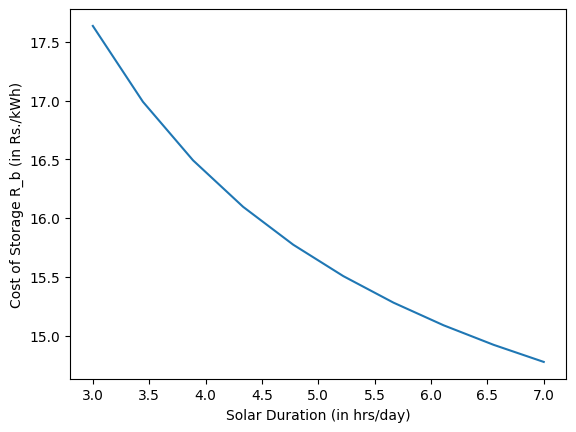
\includegraphics[height=3in]{Rb vs Ts.png}
	\caption[Optional Caption]{R\textsubscript{b} vs T\textsubscript{s} for J = Rs.20000/kWh}
	\label{fig:Ts}
\end{figure}
\newpage
\begin{figure}[H]
	\centering
	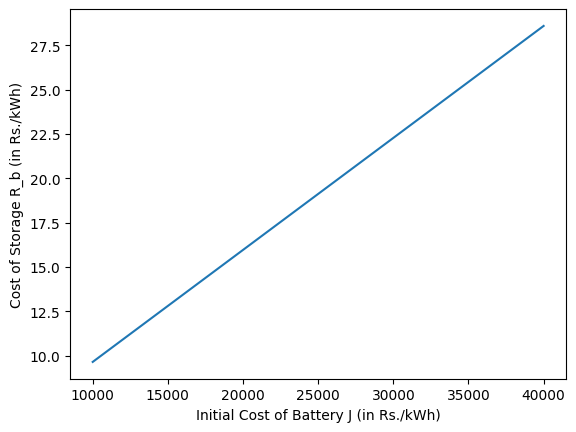
\includegraphics[height=3in]{Rb vs J.png}
	\caption[Optional Caption]{R\textsubscript{b} vs J for T\textsubscript{s} = 4.5 hrs/day}
	\label{fig:J}
\end{figure}

\section{Net Present Value and Payback Period Calculations}
We know that Net Present Value (NPV) is calculated using the formula -\\
\begin{equation}
	\text{NPV} = -C_0 - \sum_{k=1}^{n} \frac{C_k}{(1+d)^k} + \sum_{k=1}^{n} \frac{R}{(1+d)^k}
\end{equation}
where,\\
C\textsubscript{0} is the initial cost of investment\\
C\textsubscript{k} is the annual costs (including O\&M costs)\\
R is the annual revenue\\
\newline
C\textsubscript{0} in our case can be obtained by adding the initial investment costs of battery and solar setup.\\
\[
  C_0 = J \cdot C_b + K \cdot P_s
\]
\newline
Similarly, C\textsubscript{k} is obtained by taking into account the annual O\&M cost of battery (since O\&M cost of  solar PV setup is zero).\\
\[
  C_k = x \cdot J \cdot C_b
\]
\newline
Now, let us try to calculate the annual revenue. Annual revenue is the savings that we will obtain because of reduced dependence on grid.\\
Initially, before setting up the solar + battery system, the cost of using the grid per day = R\textsubscript{g}P\textsubscript{L}T\textsubscript{L}\\
After using the solar + battery system, the time for which grid will be needed is given by -\\
\[
  T_g = T_L - T_s - T_{dis}
\]
T\textsubscript{dis} is the time for which battery discharges by delivering power of P\textsubscript{L}.\\
It can be calculated as -\\
\[
  T_{dis} = \frac{\delta \cdot C_b \cdot \eta_d}{P_L} = \frac{\eta \cdot (P_s - P_L) \cdot T_s}{P_L}
\]
Here, we have substituted C\textsubscript{b} from equation (3)
\newline
Hence, the cost of using the grid per day after setting up solar + battery setup = R\textsubscript{g}P\textsubscript{L}T\textsubscript{g}\\
As a result, Annual Revenue can be written as -\\
\begin{equation}
	R = R_g P_L (T_L - T_g) d_y = R_g  T_s (P_L (1 - \eta) + \eta P_s) d_y
\end{equation}
\newline
Substituting C\textsubscript{0}, C\textsubscript{k} and R in equation (10), we get-\\
\[
  \text{NPV} = -(J C_b + K P_s) + \sum_{k=1}^{n} \frac{R - x J C_b}{(1+d)^k}
\]
Let us consider R - xJC\textsubscript{b} as net annual revenue 'R\textsubscript{n}'. Using the relation,
\[
  \frac{1}{\phi} = \sum_{k=1}^{n} \frac{1}{(1+d)^k}
\] 
where \(\phi\) is the capital recovery factor, we get,
\begin{equation}
	\text{NPV} = -(J C_b + K P_s) + \frac{R_n}{\phi}
\end{equation}
where,
\begin{equation}
  R_n = R_g  T_s (P_L (1 - \eta) + \eta P_s) d_y - x J C_b
\end{equation}
\newline
\newline
\newline
Now, we will try to calculate the Payback Period for the solar + battery setup.\\
Payback period is the number of years after which NPV becomes 0.\\
\newline
Hence, we will equate NPV to zero and first calculate the CRF '\(\phi_{pb}\)'. \(\phi_{pb}\) comes out to be \\
\begin{equation}
  \phi_{pb} = \frac{R_n}{J C_b + K P_s}
\end{equation}
\newline
We also know that Capital Recovery Factor is given by the formula -\\
\[
  \phi = \frac {d (1+d)^n}{(1+d)^n - 1} 
\]
Using this formula, substituting n = t\textsubscript{pb} and \(\phi\) as \(\phi_{pb}\), and using equation (14), we get\\
\begin{equation}
	t_{pb} = \frac{ln \frac{\phi_{pb}}{\phi_{pb} - d}}{ln (1+d)}
\end{equation} 
where d is the discount rate.\\
\newline
We will now try to plot NPV vs P\textsubscript{s} and t\textsubscript{pb} vs P\textsubscript{s}.\\
We will consider following values for the involved parameters :
(x = 0.012,
R\textsubscript{g} = Rs. 12/kWh,
\(\eta_c\) = 0.9,
\(\eta_d\) = 0.95,
eta = \(\eta_c\) * \(\eta_d\) = 0.855,
T\textsubscript{s} = 5 hrs/day,
d\textsubscript{y} = 300 days/year,
J = Rs. 20000/kWh,
\(\delta\) = 0.9,
K = Rs. 35000/kW,
P\textsubscript{L} = 40 kW,
d = 0.1)
\begin{figure}[H]
	\centering
	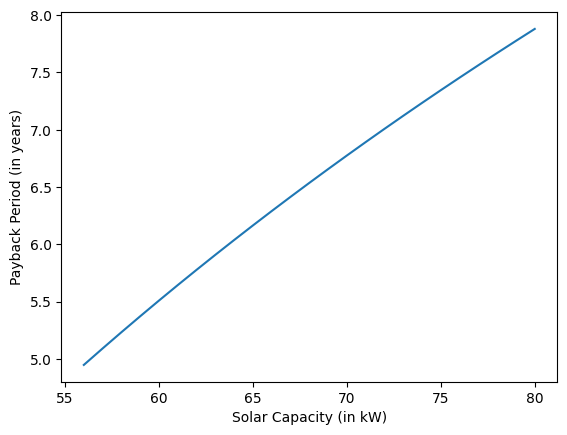
\includegraphics[height=3in]{pb vs Ps.png}
	\caption[Optional Caption]{t\textsubscript{pb} vs P\textsubscript{s}}
	\label{fig:pb}
\end{figure}
\begin{figure}[H]
	\centering
	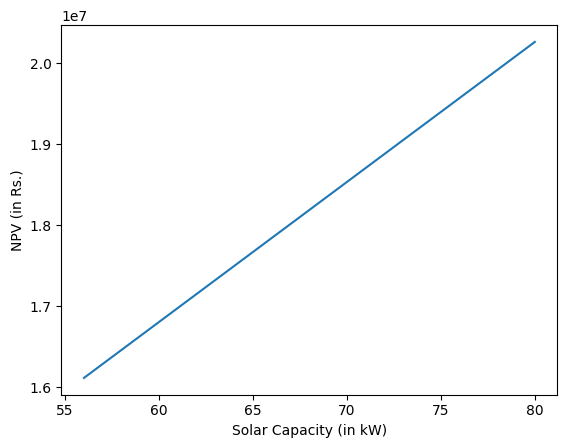
\includegraphics[height=3in]{npv vs Ps.png}
	\caption[Optional Caption]{NPV vs P\textsubscript{s} for n = 10 years}
	\label{fig:npv}
\end{figure}
Note that for plotting NPV vs P\textsubscript{s}, we have used R\textsubscript{g} as Rs. 40/kWh and not Rs. 12/kWh.\\
\end{document}
